\chapter{Capítulo 3}
Capa Límite con Difusión, Dispersión de Taylor y Flujo Turbulento con Difusión.

Este capítulo consta de las siguientes partes:
\begin{enumerate}
    \item Capa límite.
    \item Convección forzada con reacción química homogéna en una placa plana.
    \item Convección forzada  placa plana con transferencia de masa rápida.
    \item Convección forzada  placa plana con transferencia de masa lenta.
    \item Dispersión de Tayloren flujo laminar.
    \item Transferencia de masa con reacción de $1^{\text{er}}$ orden en flujo laminar turbulento.
    \item Flujo turbulento en reacción de $2^{\circ}$ orden. Mezclado turbulento.
\end{enumerate}
\section{Capa límite binaria}
Considerar un flujo binario a régimen permanente de un fluido binario. En la vecindad de la superficie sólida, las ecuaciones que gobiernan el proceso en ausencia de disipación viscosa son:
 \begin{equation}
\text{Continuidad: }\frac{\partial v_x}{\partial x} + \frac{\partial v_y}{\partial y} = 0 \label{3.1}
\end{equation}
\begin{equation}
    \begin{split}
    \text{Movimiento: } &\rho \left( v_x \frac{\partial v_x}{\partial x} + v_y \frac{\partial v_x}{\partial y} \right) =- \rho v_e \frac{\partial v_e}{\partial x} + \mu \frac{\partial^2 v_x}{\partial y^2} \\
    & + \bar{\rho} g_x \beta (T - T_{\infty}) + \bar{\rho} g_x \bar{\zeta} (w_A - w_{A\infty})
    \end{split}
    \label{3.2}
\end{equation}
\begin{equation}
    \text{Energía: } \rho \bar{C_p} \left( v_x \frac{\partial T}{\partial x} + v_y \frac{\partial T}{\partial y} \right) = 
    k \frac{\partial^2 T}{\partial y^2} - \left( \frac{\bar{H}_A}{M_A} - \frac{\bar{H}_B}{M_B} \right) r_A
    \label{3.3}
\end{equation}
\begin{equation}
    \text{Continuidad de A: } \rho \left( v_x \frac{\partial w_A}{\partial x} + v_y \frac{\partial w_A}{\partial y} \right) = 
    \rho \mathscr{D}_{AB}  \frac{\partial^2 w_A}{\partial y^2} + r_A 
    \label{3.4}
\end{equation}
donde $v_e$ es la velocidad en el límite externo de la capa límite de velocidad, $T_{\infty}$ es la temperatura en el límte externo de la capa límite térmica y $w_{A\infty}$ es la concentración másica en el límite externo de la capa límite difusional.
Los términos de flotación en la ec.(\eqref{3.2}) provenien del efecto témrico y del de concentración. En la ec.\eqref{3.3} se incluye el término de fuente de calor por reacción química. Las ecs.\eqref{3.1}-\eqref{3.4} pueden ser integrados para dar

Ecs. continuidad+movimiento:
\begin{equation}
    \begin{split}
    \mu \frac{du_x}{dy} \bigg|_{y=0} = &\frac{d}{dx} \int_{0}^{\infty} \rho v_x (v_e - v_x) dy + \frac{d v_e}{dx} \int_{0}^{\infty} \rho (v_e - u_x) dy + \rho v_o v_e + \\
   &- \int_{0}^{\infty} \rho g_x \beta (T - T_{\infty}) dy  - \int_{0}^{\infty} \rho g_x \bar{\zeta} (w_A - w_{A\infty}) dy
    \label{3.5}
\end{split}
\end{equation}

Ecs. continuidad+energía:
\begin{equation}
    k \frac{dT}{dy} \bigg|_{y=0} = \frac{d}{dx} \int_{0}^{\infty} \rho v_x \bar{C_p} (T_{\infty} - T) dy
    - \int_{0}^{\infty} \left( \frac{\bar{H}_A}{M_A} - \frac{\bar{H}_B}{M_B} \right) r_A dy
    - \rho v_{\infty} \bar{C_p} (T_{\infty} - T_0) 
    \label{3.6}
\end{equation}

Ecs. continuidad+continuidad de A:
\begin{equation}
    \rho \mathscr {D}_{AB} \frac{dw_A}{dy} \bigg|_{y=0} = \frac{d}{dx} \int_{0}^{\infty} \rho u_x (w_{A\infty} - w_A) dy
    + \int_{0}^{\infty} r_A dy - \rho v_{0} (w_{A\infty} - w_{A0})
    \label{3.7}
\end{equation}

Estas ecuaciones son extensiones de los balances de von Kármán y de la integral de momentum expuestas en el libro 1, Cap. 5.

\section{Convección forzada con reacción química homogénea en una placa plana}
\documentclass{article}
\usepackage{graphicx} % Required for inserting images
\usepackage{mathtools}
\usepackage{tikz}
\usepackage{amsmath}
\usepackage[margin=1in]{geometry}
\usepackage{caption}
\usetikzlibrary{patterns}




\title{3 Transferencia de Masa}{ 3 Transferencia de Masa}
\author{JUAN BARREIRO THIERRY}
\date{February 2025}

\begin{document}

\maketitle

\section{Convección forzada con reacción química homogénea en una placa plana}

En este caso, la concentración en la placa es $C_{A_0}$ y lejos de la placa es $C_{A_\infty}\rightarrow0$. LA reacción está dada por $R_A=-k_nC_A^n$. La concentración de A disuelta es pequeña por lo que $\mu, \rho$ y $D_{AB}$ son constantes en el fluido. EL sistema esquematizado en la figura 3.1



\centering
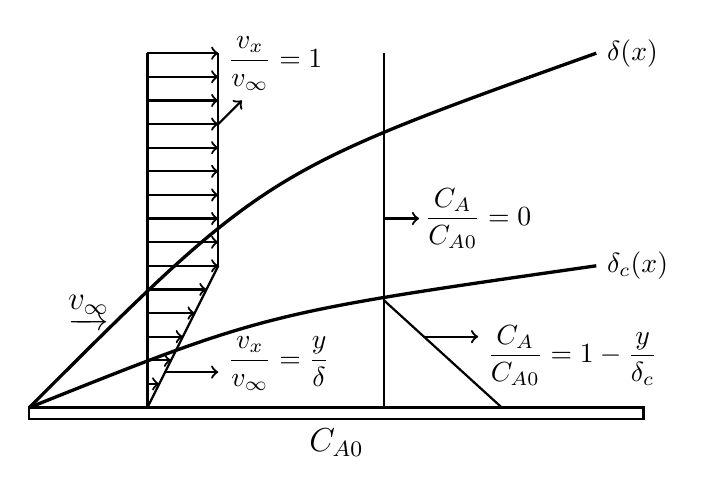
\begin{tikzpicture}[scale=3]
\draw[thick] (0,-0.05) rectangle (2.6,0);
\node[below] at (1.3,-0.05) {\large $C_{A0}$};
\draw[very thick] (0,0) .. controls (1.0,1.0) .. (2.4,1.5) node[right] {$\delta(x)$};
\draw[very thick] (0,0) .. controls (1.0,0.4) .. (2.4,0.6) node[right] {$\delta_c(x)$};
\draw[thick] (1.5,0.455) -- (2,0);
\draw[->,thick] (1.67,0.3) -- (1.9,0.3);
\node at (2.3,0.22) {$\dfrac{C_A}{C_{A0}} = 1 - \dfrac{y}{\delta_c}$};
\draw [thick] (1.5,0) -- (1.5,1.5);
\draw [->,thick] (1.5,0.8) -- (1.65,0.8);
\node at (1.9,0.8) {$\dfrac{C_A}{C_{A0}} = 0$};
\draw [thick] (0.5,0) -- (.5,1.5);
\draw[thick](0.5,0)--(0.8,0.6);
\draw[thick](0.8,0.6)--(0.8,1.5);
\node at (0.25,0.4) {\large $\underrightarrow{v_\infty}$};
\foreach \i in {0,1,...,9}
  \draw[->, thick] (0.5,{1.5 - 0.1*\i}) -- (0.8,{1.5 - 0.1*\i});
\draw[->,thick](0.5,0.5)--(0.75,0.5);
\draw[->,thick](0.5,0.4)--(0.7,0.4);
\draw[->,thick](0.5,0.3)--(0.65,0.3);
\draw[->,thick](0.5,0.2)--(0.6,0.2);
\draw[->,thick](0.5,0.1)--(0.55,0.1);
\draw[->, thick] (0.57,0.15) -- (0.8,0.15);
\node[above right] at (0.8,0.03) {$\dfrac{v_x}{{v}_\infty} = \dfrac{y}{\delta}$};
\node[above right] at (0.8,1.3) {$\dfrac{v_x}{{v}_\infty} = 1$};
\draw[->,thick](0.8,1.2)--(0.9,1.3);
\end{tikzpicture}

\label{Fig_3.1}

Fig (3.1) Perfiles de concentración y velocidad para un capa límite laminar con reacción química homogénea 


Las condiciones en la frontera son:
\begin{equation*}
    \frac{v_x}{v_\infty}|_{y\leq\delta (x)}=\frac{y}{\delta}
\end{equation*}
  \begin{equation}
      \frac{v_x}{v_\infty}|_{y\geq\delta (x)}=1
  \end{equation}
\begin{equation*}
    \frac{C_A}{C_{A_0}}|_{y\leq\delta_c(x)}=1-\frac{y}{\delta}
\end{equation*}
\begin{equation}
    \frac{C_A}{C_{A_0}}|_{y\geq\delta_c(x)}=0
\end{equation}
Definiendo $\Delta=\frac{\delta_c}{\delta}$ y suponiendo que $\Delta\leq1$ (La capa límite de concentración se encuentra dentro de la capa límite de velocidad). Además $v_o=v_y|_{y=0}\rightarrow 0$, la ecuación (3.5) se aplica al perfil de $v_x=\frac{v_\infty y}{\delta}$:
\begin{equation*}
    \mu\frac{v_\infty}{\delta}=\frac{d}{dx}\int_0^\infty \rho (v_xv_\infty-v_x^2)dy=\rho v_\infty^2 \frac{d}{dx}\int_0^\infty (\frac{v_x}{v_\infty}-\frac{v_x^2}{v_\infty^2})dy
\end{equation*}
\begin{equation}
    =\frac{d}{dx}[\rho v_\infty^2\int_0^\infty(\frac{y}{\delta}-\frac{y^2}{\delta ^2})dy]=\frac{d}{dx}\rho v_\infty^2 (\frac{y^2}{2\delta}-\frac{y^3}{3\delta ^2})|_0^\infty=\frac{d}{dx}[\rho v_\infty ^2 \delta (\frac{1}{6})]
\end{equation}
 En términos de cantidades molares, la ec (3.7) aplica a al perfil $\frac{C_A}{C_{A_0}}=1-\frac{y}{\delta_c}$   
 \begin{equation*}
     -\frac{D_{AB}C_{A_0}}{\Delta \delta}=\frac{d}{dx}\int_0^\infty v_x(C_{A_\infty}-C_A)dy+\int_0^\infty R_A dy
 \end{equation*}
\begin{equation*}
    =\frac{d}{dx}[\frac{v_\infty}{\delta}\int_0^\infty y(-1+\frac{y}{\delta _c})C_{A_0}dy]=\frac{d}{dx}[\frac{v_\infty C_{A_0}}{\delta}\delta_c^2(\frac{-1}{2}+\frac{1}{3})]
\end{equation*}
\begin{equation*}
    -\frac{D_{AB}C_{A_0}}{\Delta \delta}=\frac{d}{dx}[v_\infty C_{A_0}\delta \Delta^2(-\frac{1}{6})]+k_nC_{A_0}^n \int_0^\infty (1-\frac{y}{\delta_c})^ndy
\end{equation*}
\begin{equation}
    -\frac{D_{AB}C_{A_0}}{\Delta \delta}=\frac{d}{dx}[-\frac{1}{6}v_\infty C_{A_0}\delta \Delta^2]-\frac{k_nC_{A_0}^n}{n+1}\delta \Delta
\end{equation}
La Ec (3.10) se integra: $\frac{6\mu v_\infty}{\rho v_\infty ^2}=\delta\frac{d(\delta)}{dx}$
\begin{equation}
    \delta \frac{d}{dx}(\delta)=\frac{1}{2}\frac{d}{dx}(\delta^2) \rightarrow12\frac{\nu}{v_\infty}(x)=\delta^2
\end{equation}
Multiplicando la ec (3.11) por $-\frac{\Delta \delta}{C_{A_0}\nu}$, se obtiene:
\begin{equation*}
    \frac{D_{AB}}{\nu}=\frac{1}{6}\frac{v_\infty}{\nu}(\Delta \delta)\frac{d}{dx}(\delta \Delta^2)+\frac{k_n}{\nu}(\frac{C_{A_0}^{n-1}}{n+1})\delta^2 \Delta^2
\end{equation*}
Definiendo al número de Schmidt como $Sc=\frac{\nu}{D_{AB}}$, se obtiene:
\begin{equation*}
    \frac{1}{Sc}=\frac{v_\infty}{6\nu}(\Delta \delta)(\Delta^2\frac{d\delta}{dx}+2\Delta \delta \frac{d\Delta}{dx})+\frac{k_n}{\nu}(\frac{C_{A_0}^{n-1}}{n+1})(\frac{12\nu x}{v_\infty})(\Delta^2)
\end{equation*}
Como $\delta \frac{d}{dx}(\delta)=\frac{1}{2}\frac{d(\delta^2)}{dx}=6\frac{\nu}{v_\infty}$ y $\Delta^2\frac{d\Delta}{dx}=\frac{1}{3}\frac{d}{dx}(\Delta^3)$, luego entonces:
\begin{equation*}
    \frac{1}{Sc}=\Delta^3+\frac{v_\infty}{6 \nu}(\frac{12\nu x}{v_\infty})[\frac{2}{3}\frac{d}{dx}\Delta^3)]+12\frac{k_nC_{A_0}^{n-1}}{n+1}(\frac{x}{v_\infty})\Delta^2
\end{equation*}
\begin{equation}
    \frac{1}{Sc}=\Delta^3+\frac{4}{3}x\frac{d}{dx}(\Delta^3)+12\frac{k_nC_{A_0}^{n-1}}{n+1}(\frac{x}{v_\infty})\Delta^2
\end{equation}
Si la reacción no ocurre, entonces $k_n=0$ y la ec (3.15) se reduce a:
\begin{equation}
    \frac{4}{3}x\frac{d}{dx}(\Delta^3)+\Delta^3-\frac{1}{Sc}=0
\end{equation}
Cuya solución es:

\begin{equation*}
    \Delta^3=[c+\int \frac{1}{Sc}(\frac{3}{4x})exp(\int\frac{3}{4x}dx)dx]exp(-\int \frac{3}{4x}dx)
\end{equation*}
Donde c es la constante de integración. Efectuando las operaciones:
\begin{equation*}
    \Delta^3=[c+\frac{3}{4 Sc}\int \frac{1}{x}(x^{\frac{3}{4}})dx]x^{-\frac{3}{4}}
\end{equation*}
\begin{equation*}
    \Delta^3=\frac{c}{x^{3/4}}+\frac{3}{4Sc}x^{\frac{3}{4}}(\frac{4}{3})x^{-\frac{3}{4}}
\end{equation*}
\begin{equation}
    \Delta^3=\frac{c}{x^{\frac{3}{4}}}+\frac{1}{Sc}
\end{equation}
La constante se determina con la condición $\Delta|_{x\rightarrow 0}=finito$, que implica que:
\begin{equation}
    c=0\rightarrow\Delta= Sc^{-\frac{1}{3}}; \forall\Delta<1
\end{equation}
Esta última ecuación a su vez implica que, puesto que $\Delta\equiv\frac{\delta_c}{\delta}$, cuando no hay reacción, el cociente de los grosores de la capa límite de concentración y la capa límite de velocidad es constante. Los límites de reacción lenta y rápida pueden obtenerse a partir de la ecuación (3.13). Para reacción lenta (x pequeño), se propone la siguiente serie:
\begin{equation}
    \Delta= Sc^{-\frac{1}{3}}(1+a_1\xi+...)
\end{equation}
En donde:
\begin{equation}
    \xi=12[k_n\frac{C_{A_0}^{n-1}}{n+1}\frac{x}{v_\infty}]
\end{equation}
Substituyendo la ecuación (3.17) en la ecuación (3.13)
\begin{equation*}
    \frac{1}{Sc}=\frac{1}{Sc}(1+a_1\xi)^3+4x\Delta^2\frac{d\Delta}{dx}+\xi\Delta^2
\end{equation*}
Como $\frac{d\Delta}{dx}=\frac{d}{dx}[Sc^{-\frac{1}{3}}(1+a_1\xi)]=Sc^{-\frac{1}{3}}a_1\frac{d\xi}{dx}$ y si $x\frac{d\xi}{dx}=\xi$
\begin{equation*}
    \frac{1}{Sc}=\frac{1}{Sc}(1+a_1\xi)^3+Sc^{-\frac{2}{3}}(1+a_1\xi)^2[4Sc^{-\frac{1}{3}}a_1\xi+\xi]
\end{equation*}
\begin{equation*}
    \frac{1}{Sc}=\frac{1}{Sc}(1+a_1\xi)^3+\frac{4}{Sc}a_1\xi (1+a_1\xi)^2+\frac{Sc^{\frac{1}{3}}}{Sc}\xi(1+a_1\xi)^2
\end{equation*}
Multiplicando toda la expresión por Sc
\begin{equation*}
    1=(1+a_1\xi)+\xi(1+a_1\xi)^2(4a_1++Sc^{\frac{1}{3}})
\end{equation*}
Linealizando:
\begin{equation*}
    0=3a_1\xi+\xi(4a_1+Sc^{\frac{1}{3}})\rightarrow0=7a_1\xi+\xi Sc^{\frac{1}{3}}
\end{equation*}
Lo que implica que:
\begin{equation}
    a_1=-\frac{Sc^{\frac{1}{3}}}{7}
\end{equation}
Las ecuaciones (3.16) y (3.17) quedan así: 

Sin reacción:
\begin{equation*}
    \Delta =Sc^{-\frac{1}{3}}
\end{equation*}
Con reacción lenta:
\begin{equation}
    \Delta=Sc^{-\frac{1}{3}}(1-\frac{1}{7}Sc^{\frac{1}{3}}\xi)
\end{equation}
Donde $\xi$ está dado por en la ecuación (3.18). La ecuación (3.20) implica que el grosor de la capa límite de concentración disminuye con la reacción química.
Para una reacción rápida, se propone que $\Delta\sim \xi^{-\frac{1}{2}}$, es decir, que $\Delta=c\xi^{-\frac{1}{2}}$ en donde c es una constante. Sustituyendo esta expresión de $\Delta$ en la ecuación (3.13), se tiene:
\begin{equation*}
    \frac{1}{Sc}=\frac{4xc^3}{3}\frac{d}{dx}(\xi^{-\frac{3}{2}})+c^3\xi^{-\frac{3}{2}}+\xi c^2\xi^-1
\end{equation*}
Lo cual implica que el valor dominante de la serie a medida que $\xi$ aumenta corresponde a:
\begin{equation*}
    \frac{1}{Sc}=c^2\rightarrow c=Sc^{-\frac{1}{2}}
\end{equation*}
Y así, para $\xi$ grande:
\begin{equation}
    \Delta=(Sc\xi)^{-\frac{1}{2}}
\end{equation}
La ecuación (3.21) implica que $\frac{\delta_c}{\delta}=\frac{1}{(Sc\xi)^{-\frac{1}{2}}}$, que junto con la ecuación (3.12) revela que:
\begin{equation*}
    \delta_c=\frac{1}{(Sc\xi)^{\frac{1}{2}}}(\frac{12\nu x}{v_\infty})^{\frac{1}{2}}=\sqrt{\frac{12\nu x}{Sc\xi v_\infty}}
\end{equation*}
Cuando x es grande, $\delta_c$ es constante.
\end{document}

\section{Convección forzada en placa plana con transferencia de masa rápida}
Considerar un flujo a régimen permanente, bidimensional y de un fluido binario, como aparece en la figura \eqref{fig:Fig_3.2}.

\begin{figure}[H]
	\center
	
\includegraphics[scale=0.5]{./Capitulo3/Imagenes/Fig_3.2.JPG}
	\caption{Flujo tangencial a lo largo de una placa semi-infinita con transferencia de masa. La transición laminar-turbulenta ocurre a un Reynolds crítico $(xv_\infty / \nu)_c$ de $10^5 - 10^6$. } 
	 \label{fig:Fig_3.2}
\end{figure}

Las propiedades del fluido $\rho, \mu, \hat{Cp}, k, \mathscr{D}_{AB}$ son constantes. 

Primeramente se considerará el régimen isotérmico. 

$v_0(x)$ describe la distribución del flux de masa en la placa.

Las ecuaciones de capa límite en este caso son:

Continuidad:
\begin{equation}
	\frac{\partial v_x}{\partial x} + 		\frac{\partial v_y}{\partial y} = 0
	\label{eq_3.22}
\end{equation}

Movimiento: 
\begin{equation}
	v_x \frac{\partial v_x}{\partial x} + v_y \frac{\partial v_x}{\partial y} = \nu \frac{\partial^2 v_x}{\partial y^2}
	\label{eq_3.23}
\end{equation}

Continuidad de $A$:
\begin{equation}
	v_x \frac{\partial w_A}{\partial x} + v_y \frac{\partial w_A}{\partial y} = \mathscr{D}_{AB} \frac{\partial^2 w_A}{\partial y^2}
	\label{eq_3.24}
\end{equation}

Condiciones de frontera:
\begin{equation}
	v_x |_{y \to \infty} = v_\infty, \hspace{0.5cm} w_A | _{y \to \infty} = w_{A\infty}
	\label{eq_3.25}
\end{equation}

\begin{equation}
v_x |_{y =0} = 0, \hspace{0.5cm} w_A|_{y=0}=w_{A0}, \hspace{0.5 cm} v_y|_{y=0} = v_0 (x)
	\label{eq_3.26}
\end{equation}

Integrando la ec. \eqref{eq_3.22}:
\begin{equation}
v_y = v_0(x) - \frac{\partial}{\partial x} \int_0^y v_x dy
	\label{eq_3.27}
\end{equation}

Definiendo:
\begin{equation}
	\Pi_v = \frac{v_x}{v_\infty} \hspace{0.5cm} \text{y} \hspace{0.5cm} \Pi_w = \frac{w_A - w_{A0}}{w_{A\infty}-w_{A0}}
	\label{eq_3.28}
\end{equation}

Las ecs.\eqref{eq_3.23} y \eqref{eq_3.24} toman la forma:
\begin{equation}
	\Pi_v \frac{\partial \Pi_v}{\partial x} + \left( \frac{v_0(x)}{v_\infty} - \frac{\partial}{\partial x} \int_0^y \Pi_v dy \right)\frac{\partial \Pi_v}{\partial y} = \frac{\nu}{v_\infty} \frac{\partial^2 \Pi_v}{\partial y^2}
	\label{eq_3.29}
\end{equation}

\begin{equation}
	\Pi_v \frac{\partial \Pi_w}{\partial x} + \left( \frac{v_0(x)}{v_\infty} - \frac{\partial}{\partial x} \int_0^y \Pi_v dy \right)\frac{\partial \Pi_w}{\partial y} = \frac{\mathscr{D}_{AB}}{v_\infty} \frac{\partial^2 \Pi_w}{\partial y^2}
	\label{eq_3.30}
\end{equation}

Con condiciones de frontera:
\begin{equation}
	\Pi_v, \Pi_w |_{y \to \infty} = 1 \hspace{0.5cm} \text{y} \hspace{0.5cm} \Pi_v, \Pi_w |_{y = 0} = 0
	\label{eq_3.31}
\end{equation}

Por medio del método del combinación de variables, se propone:
\begin{equation}
	\eta = y \sqrt{\frac{1}{2} \frac{v_\infty}{\nu x}}
	\label{eq_3.32}
\end{equation}

La ec. \eqref{eq_3.29} se resuelve siguiendo la solución de Blasius. Se define la función de corriente $\Psi$ de acuerdo a: 
\begin{equation}
	v_x = \frac{\partial \Psi}{\partial y}, \hspace{0.5cm} v_y = - \frac{\partial \Psi}{\partial x}
	\label{eq_3.33}
\end{equation}

Las cuales satisfacen la ec. \eqref{eq_3.22}. Idénticamente la ec. \eqref{eq_3.23} en términos de $\Psi$ se expresa como: 
\begin{equation}
	\frac{\partial \Psi}{\partial y} \frac{\partial^2 \Psi}{\partial x \partial y} - \frac{\partial \Psi}{\partial x} \frac{\partial^2 \Psi}{\partial y^2} = \nu \frac{\partial^3 \Psi}{\partial y^3}
	\label{eq_3.34}
\end{equation}

Ahora, a partir de las ecs. \eqref{eq_3.33} y \eqref{eq_3.32}:
\begin{equation}
\Psi = \int v_x dy = \int v_x \sqrt{\frac{2 \nu x}{v_\infty}} d\eta = \int \Pi_v \sqrt{2 \nu x v_\infty} d\eta = \sqrt{2 \nu x v_\infty} f(\eta)
\label{eq_3.35}
\end{equation}

donde $f(\eta) = \int_0^\eta \Pi_v d\eta$. También a partir de la ec. \eqref{eq_3.27}:

\begin{equation}
	\Psi = - \int v_y dx = - \int \left[v_0(x) - \frac{\partial}{\partial x} \int_0^y v_x dy \right]dx = - \int v_0(x)dx + \int_0^y v_xdy
	\label{eq_3.36}
\end{equation}

Si $v_0 = 0$, recobramos la ec. \eqref{eq_3.35}. Si $v_0 \neq 0$, entonces, como $dx = \frac{-2x}{\eta} d\eta$ tenemos: 
\begin{equation}
	- \int v_0(x)dx = \frac{2x}{\eta} \int v_0(x) d\eta = \frac{2x}{y} \sqrt{2 \nu x v_\infty} \int_0^\eta \frac{v_0}{v_\infty} d\eta
	\label{eq_3.37}
\end{equation}

Luego, sustituyendo \eqref{eq_3.36} y \eqref{eq_3.37} en la ec. \eqref{eq_3.35} obtenemos:
$$\Psi = \sqrt{2 \nu x v_\infty} \left(f + \frac{2x}{y} \frac{v_0}{v_\infty} \eta \right)$$

si $v_0$ varía como $\frac{1}{\sqrt{x}}$ en \eqref{eq_3.37} tenemos que:
\begin{equation}
	\frac{2x\eta}{y} = - \sqrt{\frac{2v_\infty x}{\nu}} \hspace{0.5cm},\hspace{0.5cm} \frac{v_0}{v_\infty} \sqrt{\frac{2 v_\infty x}{\nu}} = - k  \hspace{0.5cm} \text{constante}
	\label{eq_3.38}
\end{equation}

Se requiere que $k$ sea constante, de tal forma que las velocidades o derivadas de $\Psi$ no sean función de $k$, sino de $\eta$. La ecuación de $\Psi$, por lo tanto, es:

\begin{equation}
	\Psi = \sqrt{2 \nu x v_\infty}(f-k), \hspace{0.5cm} f = \int_0^\eta \Pi_v d\eta
	\label{eq_3.39}
\end{equation}

El desarrollo de la solución de Blasius ******

\begin{multline*}
	\frac{\partial \Psi}{\partial x} = \sqrt{2 \nu v_\infty} \frac{\partial}{\partial x} (\sqrt{x} f) = \sqrt{2 \nu v_\infty x}  \frac{\partial f}{\partial x} + \frac{1}{2} x^{-1/2} f \sqrt{2 \nu v_\infty} \\
 = \sqrt{2 \nu v_\infty x} \left( - \frac{1}{2} \frac{\eta}{x} f' \right) + \frac{1}{2} f \sqrt{\frac{2 \nu v_\infty}{x}}
\end{multline*}

ya que $\frac{\partial \eta}{ \partial x} = - \frac{1}{2} \frac{\eta}{x}$

\begin{equation*}
	\frac{\partial \Psi}{\partial x} = - \frac{\eta^2}{y} \nu f' + \frac{\eta}{y} \nu f
\end{equation*}

\begin{equation*}
	\frac{\partial \Psi}{\partial y} = \frac{\partial \Psi}{\partial \eta} \frac{\partial \eta}{\partial y} = \frac{\eta}{y} \frac{\partial \Psi}{\partial \eta} = \sqrt{\frac{v_\infty}{2 \nu x}} \sqrt{2 \nu x v_\infty} f' = v_\infty f'
\end{equation*}

\begin{equation*}
	\frac{\partial}{\partial x} \frac{\partial \Psi}{\partial y} = v_\infty \frac{\partial}{\partial x} f' = v_\infty f'' \frac{\partial \eta}{\partial x} = -\frac{1}{2} \frac{\eta}{x} v_\infty f''
\end{equation*}

\begin{equation*}
	\frac{\partial^2 \Psi}{\partial y^2} = v_\infty \frac{\partial f'}{\partial y} = v_\infty \frac{\partial f'}{\partial \eta} \frac{\partial \eta}{\partial y} = v_\infty \frac{\eta}{y} f''
\end{equation*}

\begin{equation*}
	\frac{\partial^3 \Psi}{\partial y^3} = v_\infty \frac{\eta^2}{y^2} f'''
\end{equation*}

Substituyendo en la ec. \eqref{eq_3.34}:

\begin{equation*}
	(v_\infty f')\left( - \frac{1}{2} \frac{\eta}{x} v_\infty f''\right) - \left[- \frac{\eta^2}{y} \nu f' + \frac{\eta}{y} \nu f \right]v_\infty \frac{\eta}{y} f'' 
= \nu v_\infty \frac{\eta^2}{y^2}f'''
\end{equation*}

\begin{equation*}
	v_\infty f' \left( -\nu \frac{\eta^3}{y^2} f''\right) + v_\infty \frac{\eta^3}{y^2} \nu f' f'' - \frac{\eta^2}{y^2} \nu v_\infty ff'' = \nu v_\infty \frac{\eta^2}{y^2} f'''
\end{equation*}

Ya que $\frac{v_\infty}{2 x} = \frac{\eta^2}{y^2} \nu$ \\

Luego entonces:
\begin{equation}
	ff'' + f''' = 0
	\label{eq_3.40}
\end{equation}

Con las condiciones de frontera:
\begin{equation}
\begin{cases}
   f'|_{\eta \to \infty} = 1 \hspace{0.5cm} \text{(Como $v_x = \frac{\partial \Psi}{\partial y} = v_\infty f' $, significa que $v_x = v_\infty$ cuando $y \to \infty$)} \\
   f'|_{\eta =0} = 0 \hspace{0.5 cm} \text{($v_x = 0$ en $\eta = 0$)} \\
   f|_{\eta = 0} = -k \hspace{0.5cm} \text{(En la superficie $\Psi = \sqrt{2 \nu x v_\infty}(-k)$)}
\end{cases}
\label{eq_3.41}
\end{equation}

Resolviendo para $f, f', f''$ y $f'''$ es posible conocer el perfil de velocidades ($f' = v_x / v_\infty$) en función de $\eta$ para ********* de k. La solución se da por métodos numéricos.

Resultados de interés obtenidos a partir de la solución incluyen la distribución del esfuerzo cortante a lo largo de la superficie. El esfuerzo cortante sobre la supeficie está expresado por:

\begin{equation}
	\tau_0 (x) = \mu \frac{\partial v_x}{\partial y} (x,0) = \mu \frac{\partial^2 \Psi}{\partial y^2} (x,0) = \mu v_\infty \frac{\eta}{y} f'' = \mu \sqrt{\frac{v_\infty^3}{2 \nu x}} f'' (0)
	\label{eq_3.42}
\end{equation}

Adimensionalizando $\tau_0(x)$: 
	\begin{equation}
\frac{\tau_0}{\rho (v_\infty - 0) v_\infty} = \frac{\mu}{\rho}  \sqrt{\frac{1}{2 \nu x v_\infty}} f''(0) = \sqrt{\frac{\nu}{2 v_\infty x}} f''(0) = \frac{1}{\sqrt{2 Re}} f''(0)
	\label{eq_3.43}
\end{equation}

donde $Re$ es el número de Reynolds.\\

Numéricamente $f''(0) = 0.332$.\\

El mismo procedimiento se sigue para la resolución de la ec. \eqref{eq_3.30} para el perfil de concentraciones. Ahora $f' = \Pi_w = \frac{w_A - w_{A0}}{w_{A \infty} - w_{A0}}$ y análogamente a la ec. \eqref{eq_3.43} tenemos:

\begin{equation}
	\frac{j_{A0}}{\rho v_\infty (w_{A0}- w_{A\infty})} = \frac{f''(0)}{Sc} \sqrt{\frac{\nu}{2 v_\infty x}}
	\label{eq_3.44}
\end{equation}

Los perfiles de velocidad y concentración se exhiben en la figura \eqref{fig:Fig_3.2}, para diferentes valores de $k$ y del número de Schmidt ($Sc$). $k=0$ significa ausencia de transferencia de masa, $k$ positivo o negativo significa transferencia de masa hacia el fluido (evaporización) o hacia la placa (condensación), respectivamente.

\begin{figure}[H]
	\center
	
\includegraphics[scale=0.5]{./Capitulo3/Imagenes/Fig_3.2.JPG}
	\caption{Perfiles de velocidades y concentraciones en capa límite laminar sobre placa plana con transferencia de masa en la superficie} 
	 \label{fig:Fig_3.3}
\end{figure}
 %Sección 3.3
\section{Convección forzada en placa plana con transferencia de masa lenta}
 Del problema de transferencia de calor en una placa plana, se pueden derivar analogías para transferencia de masa. A partir de la expresión:

\begin{equation}
\frac{q_0}{\rho \hat{C}_p v_\infty (T_0 - T_\infty)} \approx 0.332 \, Pr^{2/3} \sqrt{\frac{\nu}{v_\infty x}}	\tag{3.45}
        \label{eq_3.45}
\end{equation}

En el caso de $k = 0$ ($v_0 (x) = 0$). De acuerdo a la ec. \ref{eq_3.43} podemos sugerir la siguiente analogía:

\begin{equation}
\frac{\tau_0}{\rho v_\infty ( v_\infty-0)} \approx \frac{q_0}{\rho \hat{C}_p v_\infty(T_0 - T_\infty)} Pr^{2/3} \approx \frac{j_{A_0}}{\rho v_\infty(w_{A_0}-w_{A_\infty})}Sc^{2/3}=  0.332 \sqrt{\frac{\nu}{v_\infty x}}
	\tag{3.46}
        \label{eq_3.46}
        
\end{equation}
\section{Difusión de Taylor en flujo laminar}
\section{Transferencia de masa con reacción de $1^{er}$ orden en flujo turbulento}


\section{Flujo Turbulento con Reacción de Segundo Orden. Mezclado Turbulento}

Considerar dos casos en los que existen dos solutos $A$ y $B$ disueltos en un solvente $S$. En el primer caso no existe reacción, y en el segundo caso se produce la reacción:
\begin{equation*}
    A + B \rightarrow \text{productos}
\end{equation*}
En ambos casos se estudia el mezclado turbulento en dos sistemas: mezclador estático (a) y dinámico (b).

\begin{figure}[h]

        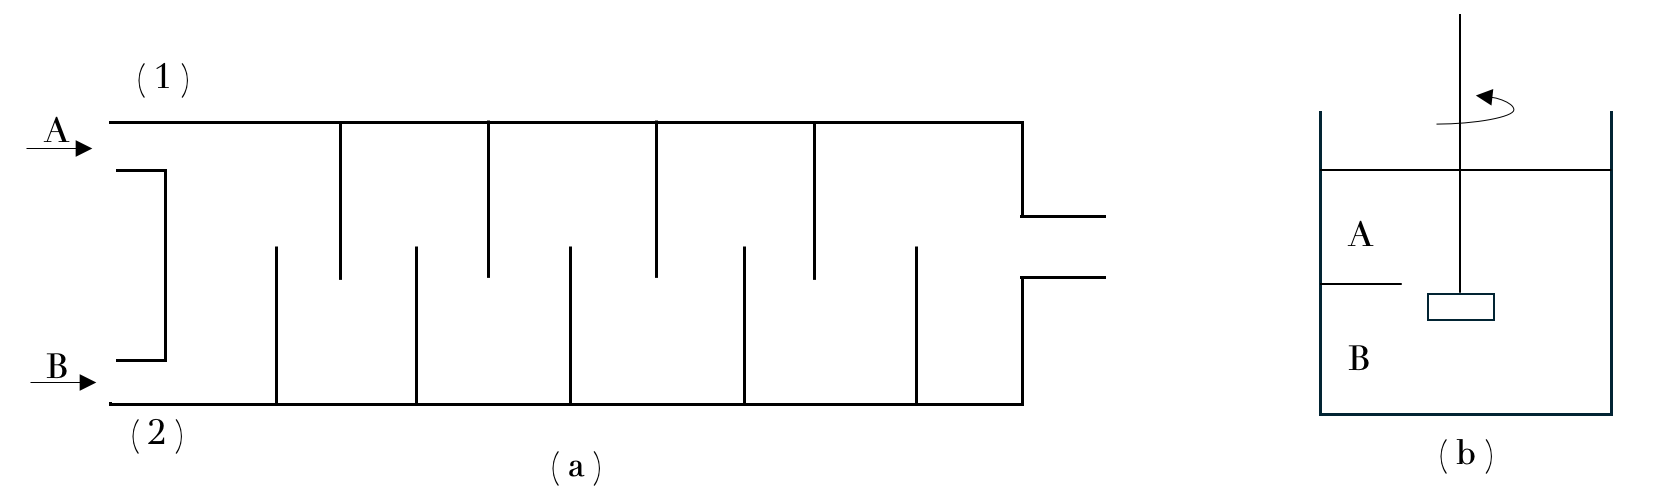
\includegraphics[width=\linewidth]{Capitulo3/Imagenes/Fig_3.8.png}
        \caption{Mezclador estático (a) y mezclador dinámico (b)}
        \label{fig:Fig_3.8}

\end{figure}
        El comportamiento de los solutos A y B se describe por medio de las siguientes ecuaciones de difusión:




\begin{equation}
    \frac{\partial C_A}{\partial t} + \underline{v} \cdot \nabla C_A = \mathscr{D}_{AS} \nabla^2 C_A + R_A
    \notag
\end{equation}

\begin{equation}
    \frac{\partial C_B}{\partial t} + \underline{v} \cdot \nabla C_B = \mathscr{D}_{BS} \nabla^2 C_B + R_B
    \label{eq_3.82}
\end{equation}




Condiciones de frontera:

\begin{equation}
    C_A = C_{A0}, \quad C_B = 0 \quad \text{para } z=0, t=0
    \notag
\end{equation}

\begin{equation}
    C_B = C_{B0}, \quad C_A = 0 \quad \text{para } z=0, t=0
\end{equation}

\subsection{Sin Reacción}

Definiendo:
\begin{equation}
    \Gamma = \frac{C_{A0} - C_A}{C_{A0}} = \frac{C_B}{C_{B0}}
\end{equation}

Las ecuaciones \eqref{eq_3.82} se reducen a:

\begin{equation}
    \frac{\partial \Gamma}{\partial t} + v \cdot \nabla \Gamma = D_{is} \nabla^2 \Gamma
\end{equation}

En las entradas (1) y (2):

\begin{equation}
    \Gamma_1 = 0, \quad \Gamma_2 = 1 \notag
\end{equation}

En flujo turbulento se propone que:

\begin{equation}
    \Gamma = \bar{\Gamma} + \Gamma'
\end{equation}

donde:
\begin{equation}
   \bar{\Gamma} = \frac{C_{A0} - \bar{C}_A}{C_{A0}} = \frac{\bar{C}_B}{C_{B0}}
\end{equation}




y $\Gamma'$ (grado de ausencia de mezclado). Restando $\Gamma$ - $\bar{\Gamma}$  y efectuando el cuadrático medio:

\begin{equation}
    \left( \frac{C_A}{C_{A0}} \right)^2 - \left( \frac{\bar{C}_B}{C_{B0}} \right)^2 = d^2
\end{equation}

En donde $d^2$ es la función de decaimiento que tiende a cero a distancias $z$ grandes o tiempos largos.


La administración de la función de decaimiento indica su dependencia funcional. Definiendo la longitud y velocidades características $l_{0}$ y $v_{0}$, obtuvimos:

\begin{equation}
    \frac{\partial\Gamma}{\partial t} + v_{b}\hat{\nabla}\Gamma = \frac{1}{Re Sc}\hat{\nabla}^{2}\Gamma  \label{eq_3.89}
\end{equation}


donde 

\begin{equation}
      \hat{t}=\frac{v_0t}{l_0}, \quad 
      \hat{v}=\frac{v}{v_0},\quad
      \hat{\nabla}=l_0\nabla, \quad
       Re=\frac{l_0v_0}{\mu}\rho 
\end{equation}

En el caso de tanques de mezclado, $l_0$ es el diámetro del impulson, $v_0=l_0N$ (N es la velocidad angular). En el caso del mezclado de dos corrientes de tubos concéntriccos \eqref{fig:Fig_3.9}, la función de decaimiento resultante se grafica en función de la distnacia axial. El mezclado a nivel molecular (micromezclado) se alcanza

\begin{figure}[h]

        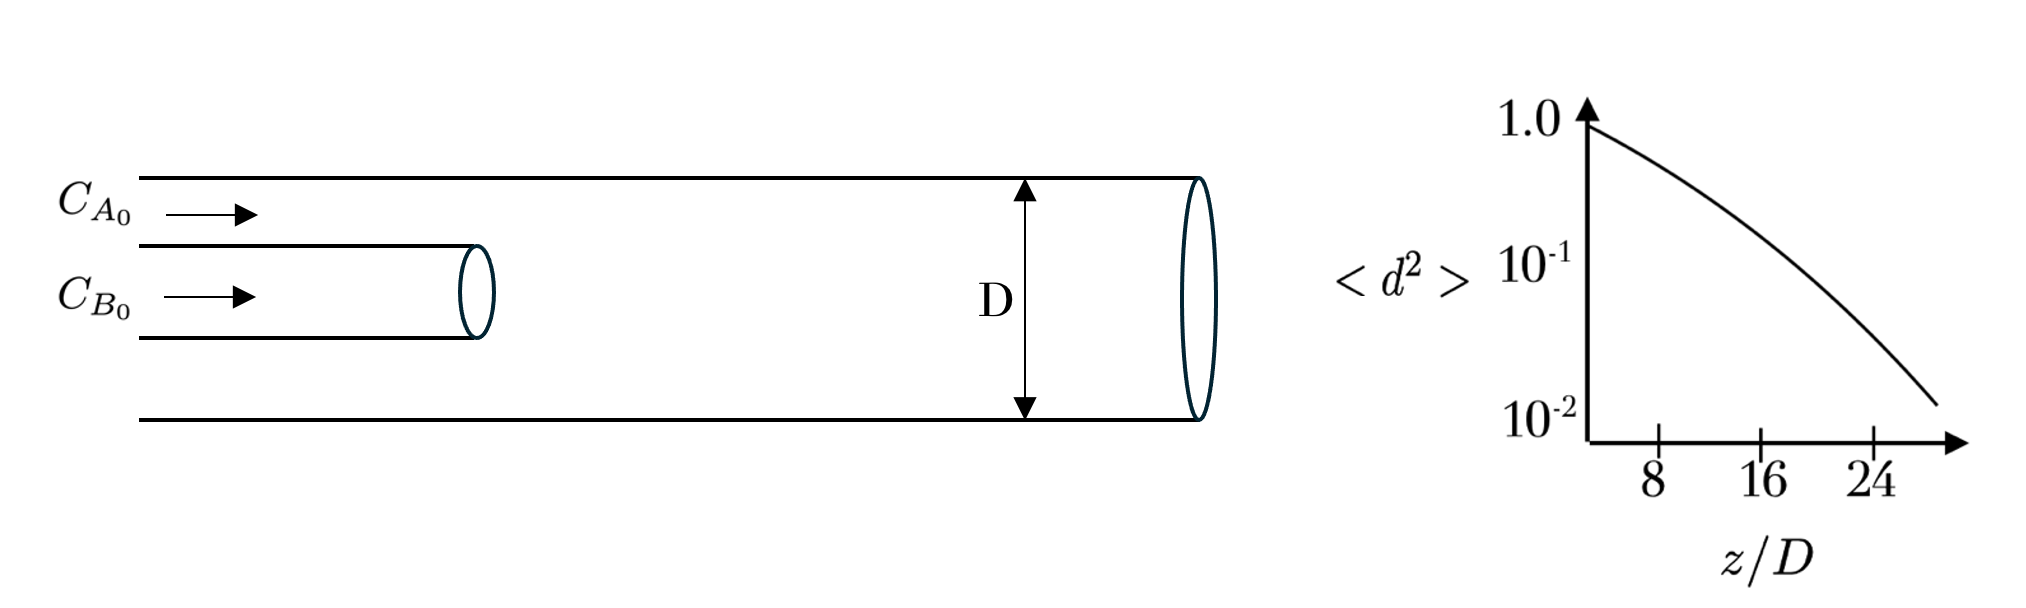
\includegraphics[width=\linewidth]{Capitulo3/Imagenes/Fig_3.9.png}
        \caption{Mezclado de 2 corrientes de A y B en tubos concéntricos y su función de decaimiento}
        \label{fig:Fig_3.9}

\end{figure}

En procesos industriales, normalamente $ReSc\sim10^9$, por lo que la ecuación \eqref{eq_3.89} se reduce a:


\begin{equation}
    \frac{\partial\Gamma}{\partial t} + v_0\hat{\nabla}\Gamma = 0
\end{equation}


Por lo que el grado de mexclado depende de $\hat{t}$ y no de $ReSc$. Como $\hat{t}=Nt_{mix}$, el producto del tiempo de mezclado $t_{mix}$ por la velocidad angular es constante, independiente de $Re$, o sea, $Nt_{mix}=K$, donde K depende de la geometría solamente.

\subsection{Con Reacción}
\begin{equation*}
    A + B \rightarrow \text{productos}
\end{equation*}
Definiendo
\begin{equation}
    \Gamma_{r}=\frac{C_{A0}-(C_A-C_B)}{C_{A0}+C_{B0}}
\end{equation}
Por la resta de las ecuaciones \eqref{eq_3.82}, la descripción del caso con reacción es la misma. Por ello:
\begin{equation}
    \left[ \frac{C_{A0}-(C_A-C_B)}{C_{A0}+C_{B0}} \right]_{reac.}=   \left[ \frac{C_{A0}-C_A}{C_{A0}}\cdot\frac{C_B}{C_{B0}} \right]_{\text{sin reac.} }
\end{equation}
que tambien es válida para las fluctuaciones.
\begin{equation}
        \left[ \frac{C_A'-C_B'}{C_{A0}+C_{B0}} \right]_{reac.}=  \left[ \frac{C_A'}{C_{A0}} \right]_{\text{sin reac.} }
\end{equation}

Esta ecuación sugiere que las fluctuaciones en $C_A$ y $C_B$ en problemas con reacción tienen lugar al mismo tiempo y escalas de distancia que los problemas sin reacción. Los casos particualres son:
\par
a) Reacción rápida: La velocidad de la reacción es controlada por difusión de las especies. Durante la escala del micromezclado, en la que la difusión es lenta en comparación con la convección, el efecto de la reacción es pequeño. En este caso tenemos:
\begin{equation}
            \left( \frac{C_A'}{C_{A0}} \right)_{reac.}=  \left( \frac{C_A'}{C_{A0}} \right)_{\text{sin reac.} }
\end{equation}
En la práctica, las reacciones rápidas son empleadas para determinar la eficiencia de los mezlcados.
\par
b) Reacciones lentas: Considerar el caso de reacciones de segundo orden irreversibles.
\begin{equation}
    R_A=-k_2C_AC_B
\end{equation}
Promediando en el tiempo: 
\begin{equation}
    R_A=-k_(\bar{C_A}\bar{C_B}+C_A'C_B')
\end{equation}
Esto indica que las fluctuaciones en $C_A$ y $C_B$ incrementan la velocidad de reacción. Por medio de un análisis de órdenes de magnitud, tenemos:
\begin{equation}
    t_A=\frac{C_{A0}}{R_A}\sim\frac{1}{k_2C_{B0}}
\end{equation}
Para una reacción rápida $t_{mix}>>t_A$ \newline
Para una reacción lenta $t_{mix}<<t_A$



\newpage
\section* {Apéndice A}
a) Transferencia de masa lenta en una placa plana. Uso de la ecuación \textbf{HACER REFERENCIA A LA ECUACIÓN 3.46}
\newline

Estimación de la velocidad de evaporación, $u_{A0}$, como función de $Sc$, del secado de una placa plana porosa saturada de agua \textbf{HACER REFERENCIA A LA FIGURA 3.2} por medio de una corriente de aire bajo condiciones tal que $W_{A0}=0.05$, $W_{A0}=0.01$ y $Sc=0.6$.
\newline
La ecuación \textbf{HACER REFERENCIA A LA ECUACIÓN 3.46} es:
\begin{equation*}
    \frac{j_{A0}}{\rho v_o(w_{A0}-w_{A\infty})}Sc^{2/3}=0.332\sqrt{\frac{\nu}{v_\infty x}}
\end{equation*}
Por medio de las ecuaciones \eqref{eq_1.24}: $n_{B0}=w_{A_0}(\underline{n}_{A_0}+\underline{n}_{B_0})+\underline{j}_{A_0}$ ya que $\underline{n}_{B_0}=0$, sustituyendo esta ecuación en la \textbf{HACER REFERENCIA A LA EC 3.46}

\begin{equation*}
    \frac{n_{A_0}(1-w_{A_0})}{\rho v_\infty (w_{A_0 }-w_{A\infty)}}=0.332Sc^{-2/3}\sqrt{\frac{\gamma}{v_\infty x}}
\end{equation*}

\begin{equation*}
n_{A_0}=0.332Sc^{-2/3}\frac{(w_{A_0}-w_{A_\infty})}{1-w_{A_0}}\rho v_\infty\sqrt{\frac{\mu}{v_\infty x \rho}}=(0.332)(0.6)^{-2/3}\frac{(0.05-0.01)}{1-0.05}\sqrt{\frac{\rho v_\infty \mu}{x}}
\end{equation*}
\begin{equation*}
    n_{A_0}=0.0196 \sqrt{\frac{\rho v_\infty \mu}{x}}
\end{equation*}
\par
b) Transferencia de momentum, calor y masa simultáneos
\newline
Las ecuaciones \textbf{HACER REFERENCIA A LA EC 3.43} y \textbf{EC 3.44} se pueden generalizar para incluir la transferencia de calor:
\begin{equation}
    \frac{q_0}{\rho \hat{C}pv_\infty(T_0-T_\infty)}=\frac{f''(0)}{Pr}\sqrt{\frac{J}{2v_\infty x}}
    \tag{A-1}
    \label{eq_A-1}
\end{equation}
Las ecuaciones \eqref{eq_A-1}, \textbf{HACER REFERENCIA A LA EC 3.43 3.44} se pueden utilizarse en las transferencias simultáneas generalizando la expresión de k \textbf{HACER REFERENCIA A LA EC 3.38}

\begin{equation}
    K=\frac{\rho_0 v_0 (x)}{\rho v_\infty}\sqrt{\frac{2v_\infty x}{\gamma}}
    \tag{A-2}
    \label{eq_A-2}
\end{equation}
donde $\rho$, $\mu$, $\hat{C}p$ y $\mathscr{D}_{AB}$ sean evaluadas a las condiciones de referencias siguientes: $T_f=\frac{1}{2}(T_0+T_\infty)$ y $W_{Af}=\frac{1}{2}(W_{A_0}+W_{A\infty})$
\newline
La resolución de problemas de transferencia simultáneas se facilita por medio de las siguientes relaciones de los fluxes:

\begin{equation*}
   R_v=\frac{(n_{A_0}+n_{B_0})(v_\infty-e)}{\tau_0} 
\end{equation*}

\begin{equation}
R_T=\frac{(n_{A_0}+n_{B_0})\hat{C}_p(T_o-T\infty)}{q_0} \tag{A-3} \label{eq_A-3}
\end{equation}

\begin{equation*}
R_w=\frac{(w_{A_0}+w_{a_\infty})(n_{A_0}+n_{B_0})}{n_{A_0}-w_{A_0}(n_{A_0}+n_{B_0})}
\end{equation*}

Los R son independientes de x y se relacionan a los números de $\Lambda=(Re,Sc,Pr)$ de acuerdo a:
\begin{equation*}
R=\frac{K\Lambda}{f''(0)} \tag{A-4} \label{eq_A-4}
\end{equation*}
\underline{Ejemplo:} Utilizar las ecuaciones \eqref{eq_A-3} y \eqref{eq_A-4} para obtener ecuaciones implícitas del flux de masa K en la superficie porosa. Para ello, se analizaran 3 casos:

\begin{figure}[h]

        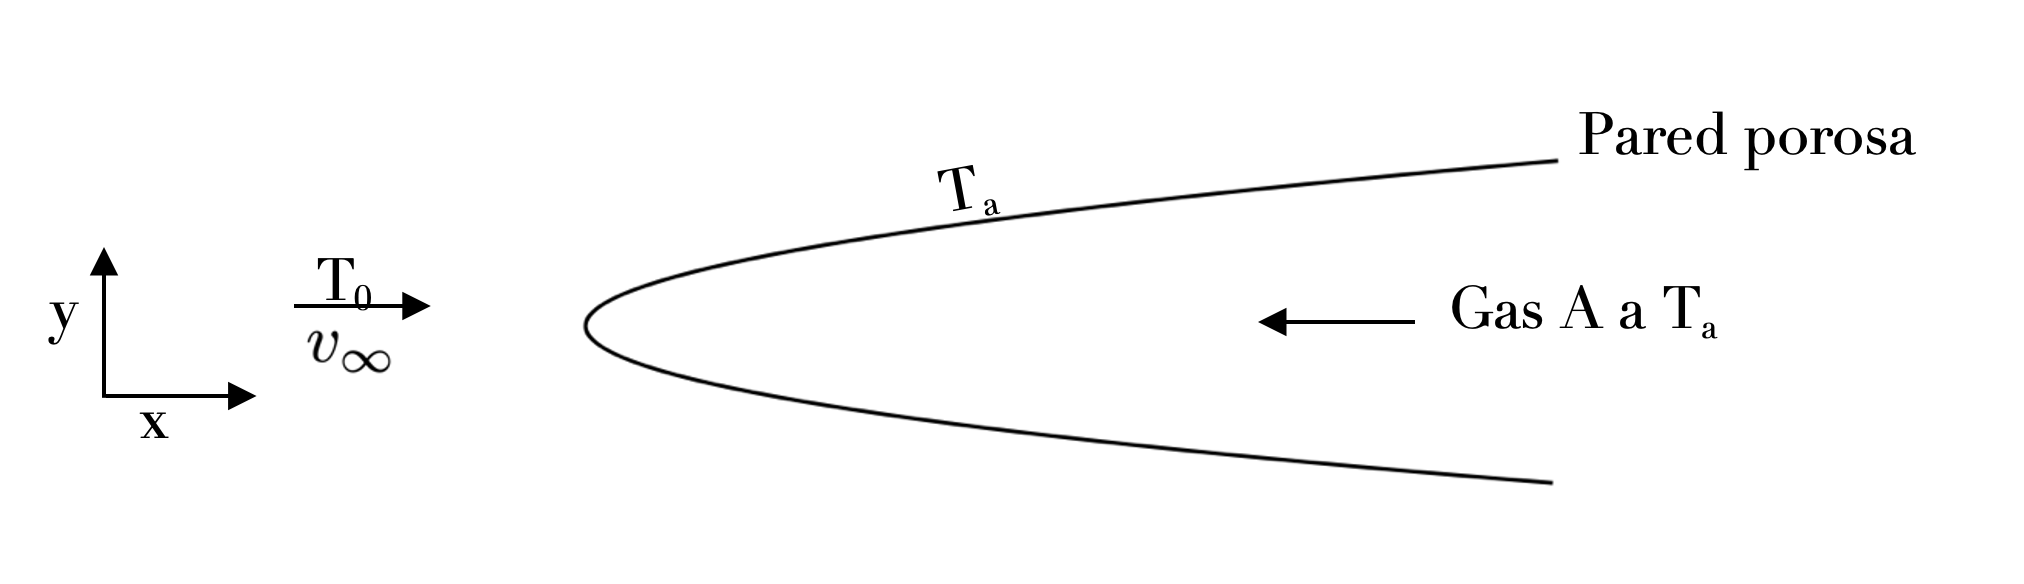
\includegraphics[width=\linewidth]{Capitulo3/Imagenes/Fig_A.1.png}
    \caption{Enfriamiento por transpiración en una placa porosa.}
        \label{fig:Fig_A.1}

\end{figure}

\begin{enumerate}
    \item Evaporación de un líquido A en una corriente de A y B. B es insoluble en A. \newline
    Como $n_{B_0}=0$, $R_w$ en \eqref{eq_A-3} se puede calcular: $R_w=\frac{w_{A_0}-w_{A\infty}}{1-w_{A_0}}$, donde $K=\frac{R_w f''(0)}{Sc}=\frac{1}{Sc}\frac{w_{A_0}-w_{A\infty}}{1-w_{A_0}}f''(0)$
    \item Reacción irreversible de A (gas) en C (sólido) $\to$ B (gas) de acuerdo a $A+C\to 2B$. Pesos moleculares de A y B son iguales. Como $n_{B_0}=-2n_{A_0}$ y $w_A=0$, $R_w=\frac{0-w_{A_\infty}}{-1}=w_{A_\infty}$, donde $K=\frac{1}{Sc}w_{a_\infty f''(0)}$
    \item Enfriamiento por transpiración. Gas A solamente
    \newline 
    Balance de energía:
    \begin{equation*}
        q_0=v_0\hat{C}_p\rho_0(T_a-T_0 )=n_{A_0}\hat{C}_p(T_a-T_0)
    \end{equation*}
    De las ecuaciones \eqref{eq_A-3}: $R_T=\frac{n_{A_0}\hat{C}_p(T_o-T\infty)}{n_{A_0}\hat{C}_p(T_a-T_0)}$
    \newline
    El valor de \( K \) es: \[ K = \frac{1}{Pr} \left( \frac{T_0 - T_\infty}{T_a - T_0} \right) f''(0) \]
\end{enumerate}
